\section{Motifs, fields and folded closure}
\label{sec:motif-field-folding}
\label{sec:curl-closure-duon-current}
\subsection{Curl forms}
\label{subsec:curl-closure}
\subsubsection{Curl}
\label{subsec:curl}
\begin{definition}[Curl. \appref{app:cc-curl}]
Curl is returned closure through a hinge on its certified support. A\(\Omega\)D calculates its hinge return, reclosure, duration, orientation, and returned current on declared windows.
\end{definition}

\subsubsection{Nested curl}
\label{subsec:nested-curl}
\begin{definition}[Nested curl. \appref{app:cc-nested-curl}]
A nested curl is a curl carried inside another curl.
\end{definition}

\subsubsection{Pin-curl}
\label{subsec:pin-curl}
\begin{definition}[Pin-curl. \appref{app:cc-pin-curl}]
A pin-curl is a returned curl whose residue seats, delays, or fixes a hinge.
\end{definition}

\subsubsection{Curling curls}
\label{subsec:curling-curls}
\begin{definition}[Curling curls. \appref{app:cc-curling-curls}]
Curling curls are recursive returns that become active path structure inside the fractal tesseract topology.
\end{definition}

\subsection{Dion}
\label{subsec:dion}
\begin{definition}[Dion. \appref{app:cc-dion}]
A dion is an oriented two-position branch pattern around the retained monon hinge. Its compressed signature is
\[
D_\alpha=(+1,-1),\qquad D_\Omega=(-1,+1).
\]
\end{definition}

\subsection{Duon}
\label{subsec:duon}
\begin{definition}[Duon. \appref{app:cc-duon-duad-cycle}]
A duon is Dion--hinge--Dion returned-current support. A compact unresolved form is
\[
\mathrm{duon}=D_i\Box D_j,
\qquad D_i,D_j\in\{D_\alpha,D_\Omega\}.
\]
A resolved duon carries the monon hinge / pivot value:
\begin{equation}
D_i\mu_M D_j,
\qquad
D_i,D_j\in\{D_\alpha,D_\Omega\},
\qquad
\mu_M\in\{-1,0,+1\}.
\label{eq:duon-current}
\end{equation}
\end{definition}

\subsubsection{Current cell}
\label{subsec:duon-current-cell}
A duon current is carried hinge-current through cycle support. The primitive resolved family has
\[
2\times3\times2=12
\]
variants. Duon, duad, and temporal cycle presentation. \appref{app:cc-duon-duad-cycle}.

\paragraph{Finite unspooling chart.}
\label{subsec:finite-q4-witness}
In the inherited finite chart, a resolved Duon has four active Dion positions
and one carried monon hinge. Declaring a retained/unspooled marker at each of
the four positions gives the chart \(\{0,1\}^4\); one-marker updates have
Hamming distance one. The marker independence is a declared chart convention,
not an extra primitive distinction or a proof that all chart words are admitted
Duon motifs. The twelve oriented Dion--pivot--Dion variants in
\eqref{eq:duon-current} are a separate grammar count.

\subsubsection{Branch/hinge/branch reflection duration}
\label{subsec:branch-hinge-rd}
Reflection duration is counted on branch/hinge/branch return support. For a returned-current path history \(\gamma\) on \(B\),
\begin{equation}
RD_\gamma(B)
=
\Pi^-_\gamma(B)
+
H_{\mu,\gamma}(B)
+
\Pi^+_\gamma(B).
\label{eq:branch-hinge-rd}
\end{equation}
Here \(\Pi^-_\gamma\) is the first-branch support, \(H_{\mu,\gamma}\) is the hinge recurrence contribution, and \(\Pi^+_\gamma\) is the reflected return-branch support. If the branch supports are symmetric, \(\Pi^-_\gamma=\Pi^+_\gamma=\Pi\), then
\begin{equation}
RD_\gamma(B)=2\Pi+H_{\mu,\gamma}(B).
\label{eq:branch-hinge-rd-symmetric}
\end{equation}
The familiar \(RD=2\Pi+1\) is the single-hinge reduction \(H_{\mu,\gamma}=1\), not a universal hinge rule. For a retained cycle \(C\) on \(B\), write the reflection-duration accessor as
\[
RD_B(C)=\Pi^-_B(C)+H_{\mu,B}(C)+\Pi^+_B(C).
\]
RD counts declared branch/hinge support occurrences. It is a support accessor; directional coupling and scalar duration have their separate interfaces in Section~\ref{sec:wave-state-relational-time}.

\subsection{Duad}
\label{subsec:duad}
\begin{definition}[Duad. \appref{app:cc-duon-duad-cycle}]
A duad is the seat-taken state of the same duon current.
\end{definition}


\paragraph{Admission binding.}
The complete admitted motif record is
\begin{equation}
\begin{split}
K_{\mathrm{adm}}(B,i;\mathrm{cert})={}&
(i,s_{\mathrm{core}},\mathcal C_L,\chi_\mu,\mathbf a,r,\sigma^C_B,\\
&HT(K;i,B),\operatorname{Cert}(K;i,B)).
\end{split}
\label{eq:motif-admission}
\end{equation}
The registry binds motif identity, scope, lineage, exact trace digest,
closure witness/status and certificate digest. Unknown, empty or mismatched
records fail validation before model or harmonic use. A core signature is
syntax until its construction witness is bound. Enclosure, chirality and
scalar RD do not replace lineage. Equal scalar values can accompany distinct
motifs. A certificate validates a witnessed construction, rather than
manufacturing it from a name.
The primitive component constructor uses the same scope, lineage and resolution
for its component and target traces. Cross-scale folding carries its separately
declared scope map and inner identities as in \eqref{eq:fold-outer-closure}.
Every component trace is bound to its certificate and must be committed before
the construction step that consumes it. The constructed motif's returned current
and its distinct later recurrence use this same evidence; a Duad changes seating
status of the Duon current while retaining its identity.
\begin{equation}
\mathrm{Dimonon}=2\,\mathrm{Monon}\ne\mathrm{Dion},\qquad
\mathrm{Duon}=D_i\mu_M D_j.
\label{eq:motif-grammar}
\end{equation}
The carried monon pivot \(\mu_M\) and its state are distinct from omission of
the mandatory temporal hinge. Dion endpoint adjacency never licenses a direct
temporal branch reversal. Duad names a seated state of the same Duon current;
a generic two-cycle \(C_2\) supplies neither the Duon grammar nor its witness.
Standalone trion names the threefold core unit; \(3:j\) composes \(j\) such
units with inherited construction provenance.

\subsection{Curling-curl support forms}
\label{subsec:curling-curl-support-forms}

A compact expression \(p{:}q{:}L\) is a compressed curling-curl specification. The \(p{:}q\) part names the retained curling-curl support form, the construction trace admits it on \(B\), and \(L\) declares the enclosure/window support used by a downstream entry. In the single-hinge symmetric fixture,
\[
\Pi(p{:}q)=q^p+q,
\qquad
RD_B^{(1)}(p{:}q)=\Pi(p{:}q)+1+\Pi(p{:}q).
\]
Thus \(1{:}2\) gives \(\Pi=4\) and \(RD_B^{(1)}=9\); \(3{:}2\) gives \(\Pi=10\) and \(RD_B^{(1)}=21\); \(3{:}3\) gives \(\Pi=30\) and \(RD_B^{(1)}=61\); \(3{:}4\) gives \(\Pi=68\) and \(RD_B^{(1)}=137\). These are internal reflection-duration accessors of declared curling-curl specifications. The live calculus keeps the construction trace, isotropic/anisotropic Markov choice, hinge slide, jitter, boundary capacity, and admission status visible. Measured-sector interpretations, if any, belong to the manual external-comparison layer.

\begin{definition}[Support expression]
A support expression is formal syntax
\begin{equation}
\Sigma=(s_1,\ldots,s_m;L),
\label{eq:support-expression}
\end{equation}
where each \(s_i=p_i{:}q_i\) and \(L\) is an optional shared enclosure qualifier.
\end{definition}

\begin{definition}[Curling-curl support form]
A curling-curl support form is the retained recursive curl/cycle form proposed by a support expression and admitted on a declared boundary/window after its construction trace is declared or inherited.
\end{definition}

A compact expression such as \(1{:}2{:}6\), \(3{:}3{:}6\), or \(3{:}4{:}6\) proposes a specification \(K_{\mathrm{prop}}\). Admission is a traced calculation on the declared scope:
\begin{equation}
K_{\mathrm{prop}}
\xrightarrow{\,HT(K;B)\,}
K_{\mathrm{adm}}(B).
\label{eq:key-proposed-admitted-trace}
\end{equation}
Here \(HT(K;B)\) is the construction trace of the proposed specification on \(B\). The specification \(K_{\mathrm{prop}}\) does not by itself determine closure, pressure, shedding, or a measured-sector comparison label. Those are formed from the declared trace on \(B\).

The downstream value construction is given in \eqref{eq:support-trace-spine}, after its duration, pressure and response interfaces.


The following are compact curling-curl specifications. Their admitted status, closure, hinge, pressure, and shedding are certified only by \(HT(K;B)\):
\[
1{:}2{:}6=\text{Dimonhexon}
=\text{Dimonon curling-curl support form carried on }C_6,
\]
with nesting, hinge, and closure details supplied by \(HT(1{:}2{:}6;B)\). Similarly,
\[
3{:}3{:}6=\text{Tritriohexon},
\qquad
3{:}4{:}6=\text{Tetratriohexon},
\]
are curling-curl support forms carried on \(C_6\); closure status is a construction-trace assertion, not a bare naming fact. SADAR couples retained curling-curl beats after admission.

\aodprovenance{\eqnref{eq:cycle-valued-field-compression}, \eqnref{eq:branch-hinge-rd}, \eqnref{eq:sadar-operator-cycle}.}

\subsection{Scoped field organization}
\label{sec:field}
\label{sec:field-disposition}
\label{subsec:declared-field-choice}
A field organizes admitted recurrent wave identities at a declared scope:
\begin{equation}
F_{B,\lambda}|_k=(B,\lambda,I_B(k),
\{W^{\mathrm{id}}_{B,i}\}_{i\in I_B(k)}).
\label{eq:field-organization}
\end{equation}
Here \((B,\lambda)\) is field identity and \(I_B(k)\) is present membership.
Member state remains in \(S^W\), not in the identity. Alias resolution maps
names to this record and then to unique wave identities; two aliases of one
wave do not supply two cadences. Existing certificates validate membership.
That validation adds no closure, recurrence or wavehood.
\begin{equation}
C^{\mathrm{ret}}=\text{retained closure lineage},\qquad
\operatorname{Resolve}(F_{B,\lambda})=\{W^{\mathrm{id}}_{B,i}\}_{i\in I_B}.
\label{eq:retained-lineage-field-separation}
\end{equation}
\paragraph{Memorum.}
\label{subsec:field-memorum}
The organization exposes members' retained predecessor closures, present
boundaries and successor horizons. Finer wave organizations can be retained
inside it. Their membership and evidence persist when a next enclosing scope
is proposed.
\subsubsection{Region}
\label{subsec:field-region}
\begin{definition}[Region]
A region is a declared retained part of a field. Regions carry current, closure, pressure, and returned-current orientation.
\end{definition}

\subsubsection{Boundary}
\label{subsec:field-boundary}
\begin{definition}[Boundary]
A boundary is the retained interface of a declared region or field. Boundary accounting records current and closure across the boundary.
\end{definition}

\subsubsection{Tesseract-admissible field boundary}
\label{subsec:tesseract-admissible-boundary}
When a retained field boundary is induced by the finite \(Q_4\) Hamming--1 support, write \(\partial_TF\) and use
\[
B=(\partial_TF,\omega).
\]
The finite Hamming--1 support is derived in \secref{subsec:four-edge-x-witness}; its tesseract-admissible boundary is defined by \eqref{eq:tesseract-admissible-boundary}.

\subsubsection{Polychiral shell dressing}
\label{subsec:polychiral-shell-dressing}
\begin{definition}[Polychiral shell dressing]
A polychiral shell dressing is field outer dressing. It carries Capital-Alpha/Omega return orientation, polarization imbalance, return duration, pressure, and SADAR coupling.
\end{definition}

Tritrio::Tetratrio::hexon. \appref{app:cc-basic-shared-hexon}. Dimonhexon. \appref{app:cc-standalone-enclosed-names}.

\begin{figure}[H]
\centering
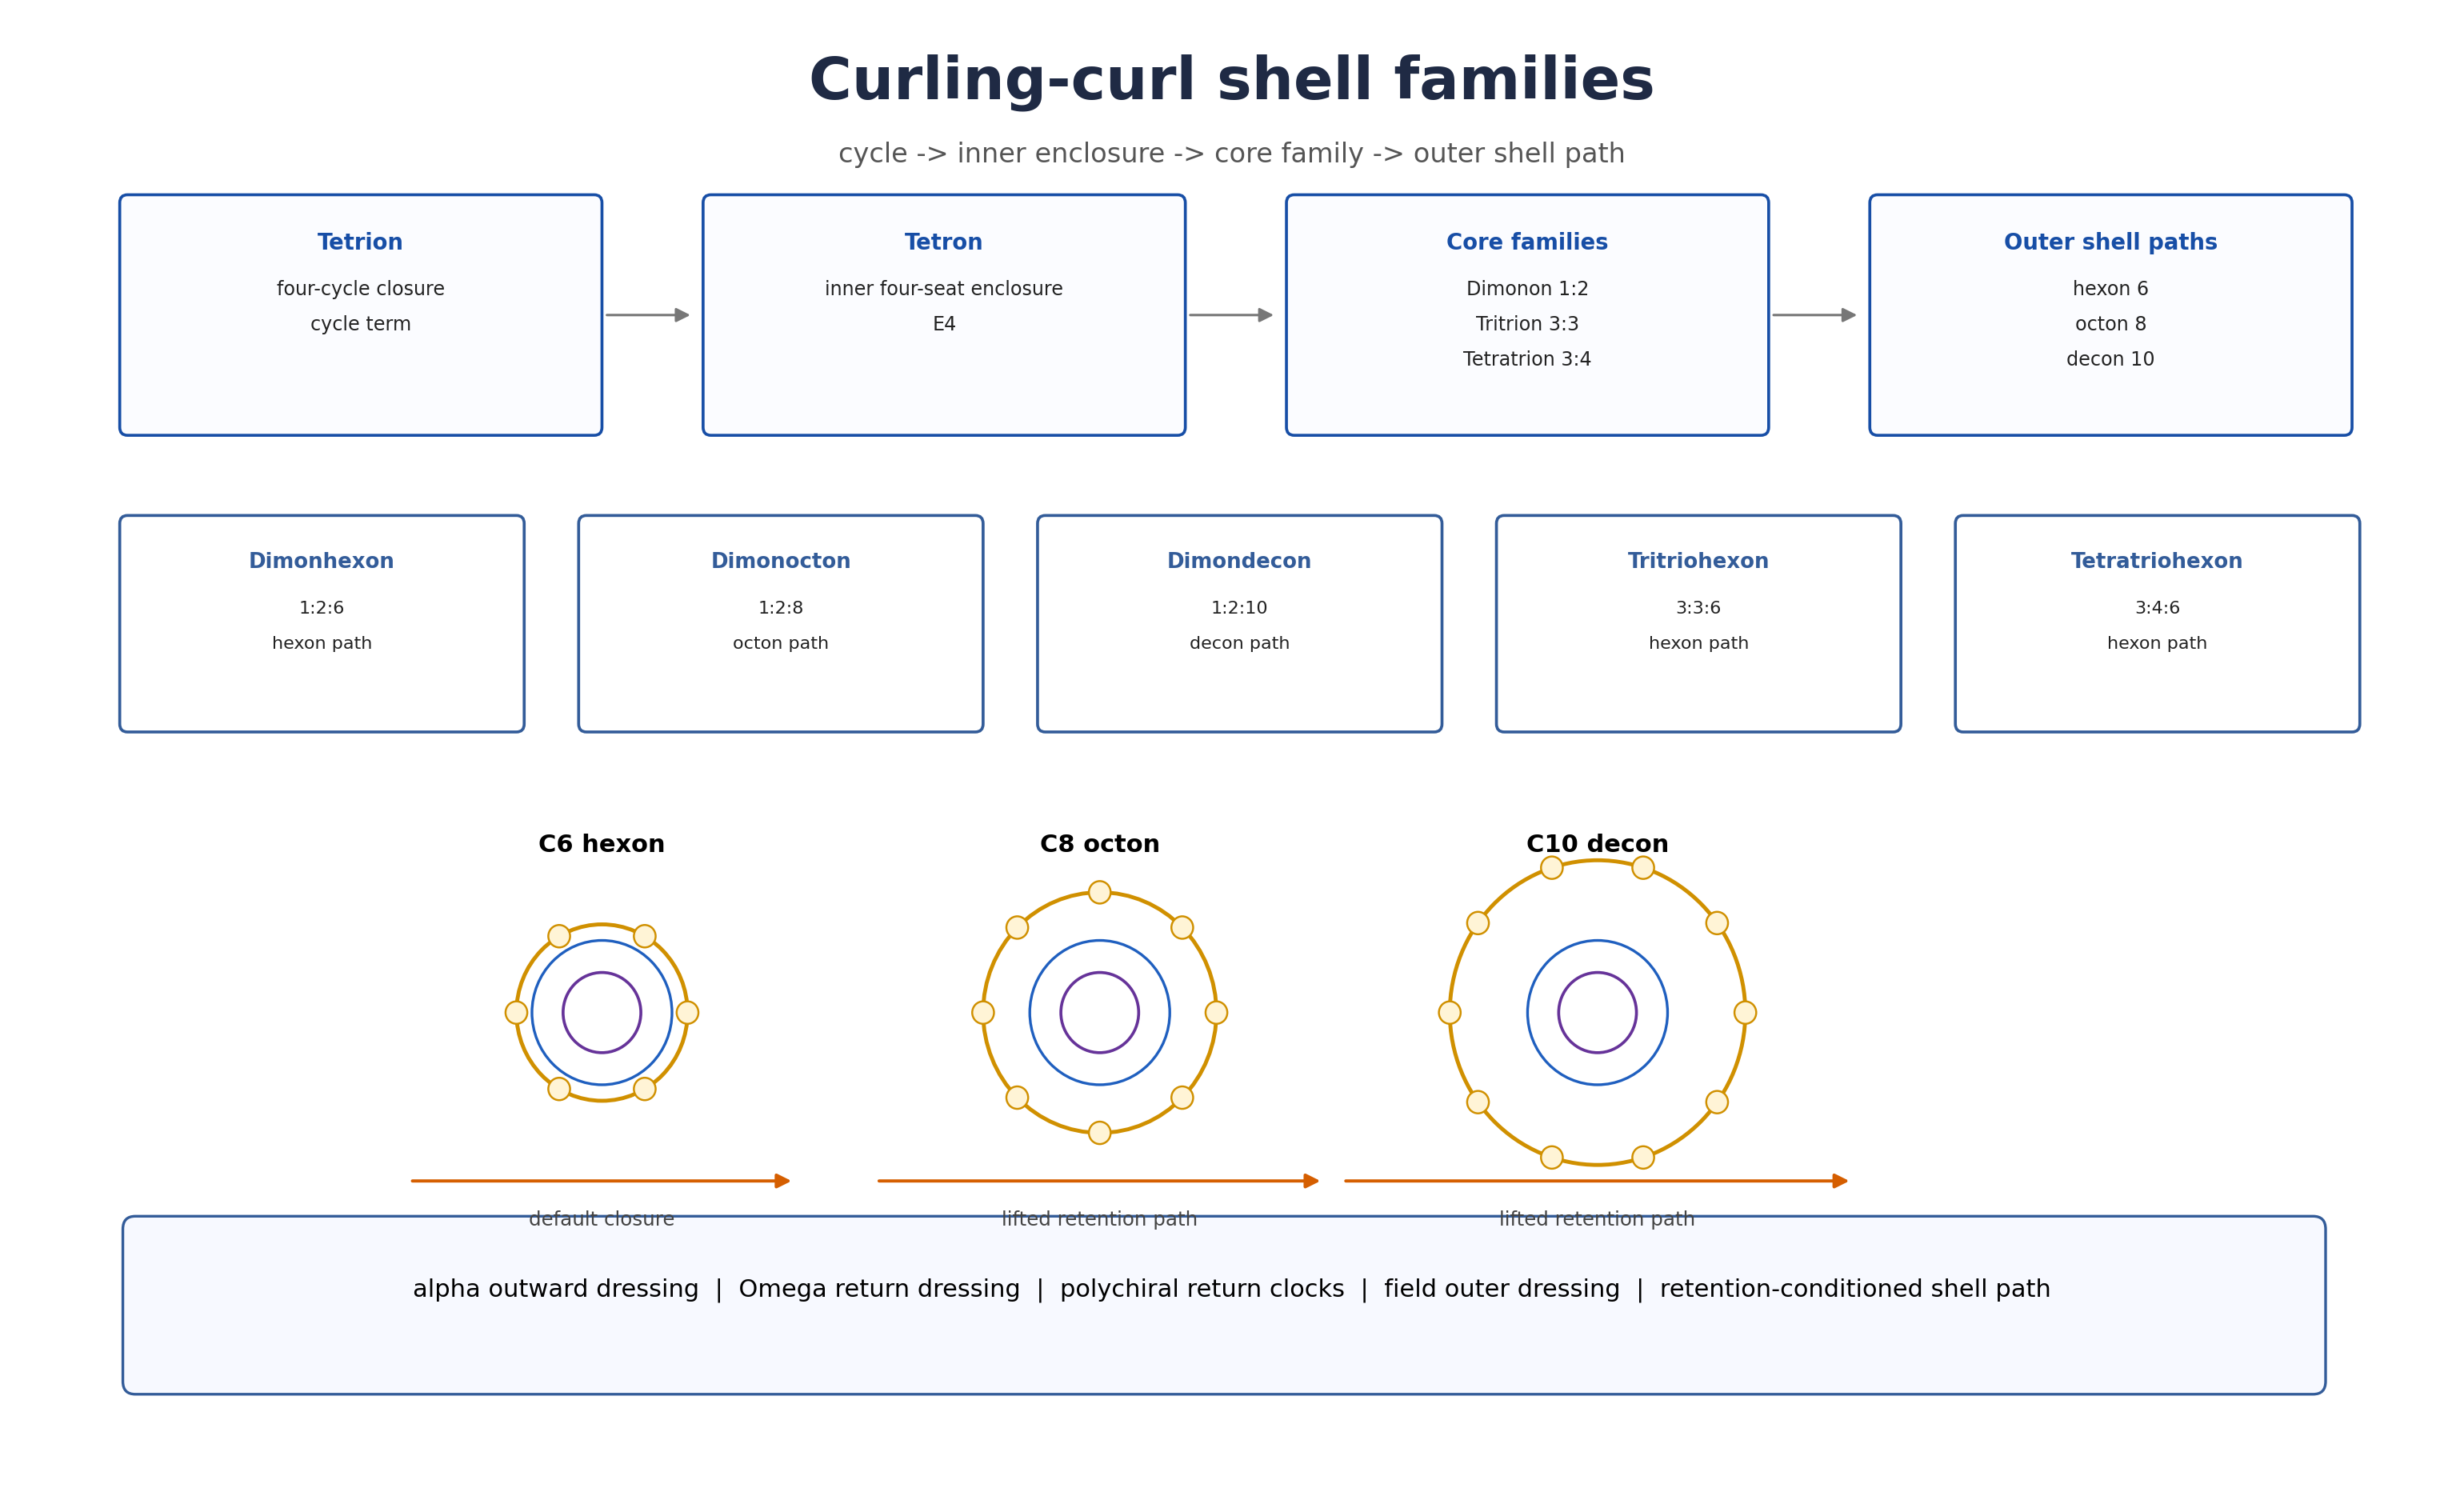
\includegraphics[width=0.96\linewidth]{figures_jpg/curling_curl_layers.png}
\caption{Curling-curl shell families.}
\label{fig:curling-curl-shell-families}
\end{figure}

\paragraph{Support-enclosure integrity.}
A tetron is \(E_4\): the default inner enclosure with four seats. Hexon, octon, and decon name outer shell paths. \appref{app:cc-support-enclosure-names}. A boundary can cut through a retained enclosure for accounting. That partial boundary is a sample of the enclosure structure. The complete enclosure identity follows the retained even-address topology.

\subsection{Folded outer closure}
\label{subsec:field-as-monon-compression}
For a proposed next-scope boundary enclosing retained wave organization \(\mathcal F\), a successful outer trace and certificate bind one completed outer closure:
\[
\mathrm{monon}_{\mathcal F}=\operatorname{cycle}_{\partial\mathcal F}(x\succ x=x).
\]
The internal field may contain curls, shells, temporal cycle presentations, returned-current duration, pressure, and SADAR. The outer witness binds the whole retained complex as one closure; later distinct outer reclosure supplies recurrence at that scope.


\subsection{Cycle-valued field compression}
\label{subsec:cycle-valued-field-compression}
\begin{definition}[Cycle-valued field compression]
Let \(f=\partial_T\mathcal F\) be a tesseract-admissible boundary and let \(B_f=(f,\omega_f)\). For an internal support expression \(\Sigma\), the certified cycle-valued compression, conditional on an actual outer return witness, is
\begin{equation}
C_f[\Sigma]_{\AO}
:=
\operatorname{cycle}_{\partial_T\mathcal F}
\left[
  x\succ x=x;\ \operatorname{int}=\Sigma,\ \omega_f
\right]_{\AO}.
\label{eq:cycle-valued-field-compression}
\end{equation}
The enclosing closure binds one next-scope phase; the boundary alone supplies a proposal. The internal support expression remains carried as cycle provenance.
\end{definition}


\paragraph{Fold and exposure.}
\begin{equation}
\{C^{\mathrm{ret}}_{B_\ell,i}\}_i
\xrightarrow{\operatorname{Fold}^{\uparrow}}K^{\mathrm{prop}}_{B_{\ell+1}}
\xrightarrow{\mathrm{OuterClose}+\mathrm{OuterCert}}C^{\mathrm{ret}}_{B_{\ell+1}}.
\label{eq:fold-outer-closure}
\end{equation}
Contact, adjacency, superposition and mixing can propose an outer structure.
The proposal binds the exact inner identities, their certificates and the map
from each inner scope to the proposed outer scope. The outer certificate commits
that construction witness; attaching an unrelated higher-scale loop afterward
does not establish the fold. Each consumed inner input precedes its consumption.
The certified outer closure contributes one phase. Its distinct compatible
outer reclosures are required for an outer wave and then field organization.
\begin{equation}
\operatorname{Expose}^{\downarrow}(C^{\mathrm{ret}}_{B_{\ell+1}})
=\{C^{\mathrm{ret}}_{B_\ell,i},\mathrm{lineage},\mathrm{orientation},
\mathrm{history},\mathrm{certificates}\}_i.
\label{eq:expose-inner-lineage}
\end{equation}
For an outer wave the same exposure additionally returns each inner wave,
cadence, self-separation, current and memory. Outer shedding preserves
surviving certified inner closures and waves. Inner beats cannot be reused as
new outer returns. Fusion applies this closure construction to a folded
complex; its pressure-resolved routing model is derived in Section~\ref{sec:fusion-closure-chain-reclosure}.

The scalar reflection-duration value is an A\(\Omega\) accessor of the cycle-valued object. For a single support \(p{:}q\),
\begin{equation}
RD_{\AO}\!\left(C_f[p{:}q];B_f\right)
=
\Pi^-_f(p{:}q)+H_{\mu,f}(p{:}q)+\Pi^+_f(p{:}q).
\label{eq:cycle-rd-accessor}
\end{equation}
The scalar accessors \(RD_{\AO}\), \(\rho^D_\omega\), \(P^D\), and \(Q^D\) are obtained from \(C_f[\Sigma]_{\AO}\) only after the declared cycle-valued field compression is fixed. These scalar accessors do not replace the cycle-valued field compression.

\subsection{Alpha--Omega hinge kernel}
\label{subsec:ao-kernel}
\begin{definition}[Alpha--Omega hinge kernel]
The explicit hinge presentations are
\begin{align*}
A\leftrightarrow_{\mu}\Omega
&:=
\text{Alpha/Omega branch order through hinge }\mu,\\
\Omega\leftrightarrow_{\mu}A
&:=
\text{Omega/Alpha branch order through hinge }\mu.
\end{align*}
For a retained cycle \(C\), define the compact branch/hinge/branch operators
\begin{equation}
\mathsf{AO}_{\mu}(C)
:=
\operatorname{A\leftrightarrow_{\mu}\Omega}(C)
=
\left\langle
\Pi_\alpha(C),
H_\mu(C),
\Pi_\Omega(C)
\right\rangle.
\label{eq:ao-kernel}
\end{equation}
\begin{equation}
\mathsf{OA}_{\mu}(C)
:=
\operatorname{\Omega\leftrightarrow_{\mu}A}(C)
=
\left\langle
\Pi_\Omega(C),
H_\mu(C),
\Pi_\alpha(C)
\right\rangle.
\label{eq:omega-alpha-hinge-kernel}
\end{equation}
The hinge \(\mu\) supports handed return. The chirality tag records the branch-order orientation:
\begin{equation}
\chi_\mu(C)=+1
\Longleftrightarrow
C:A\leftrightarrow_{\mu}\Omega,
\qquad
\chi_\mu(C)=-1
\Longleftrightarrow
C:\Omega\leftrightarrow_{\mu}A.
\label{eq:hinge-chirality-tag}
\end{equation}
The hinge flip exchanges the branch order:
\begin{equation}
\operatorname{flip}_\mu(A\leftrightarrow_{\mu}\Omega)=\Omega\leftrightarrow_{\mu}A,
\qquad
\operatorname{flip}_\mu(\Omega\leftrightarrow_{\mu}A)=A\leftrightarrow_{\mu}\Omega.
\label{eq:hinge-chirality-flip}
\end{equation}
The compact qualifier \(\AO\) marks the Alpha--Omega hinge presentation in subscripts, as in \(C_f[\Sigma]_{\AO}\). The forms \(A\Omega\) and \(\Omega A\) are implicit-hinge shorthand only after the explicit hinge presentation has been declared.
The \(\Omega\)-branch is closure-subservient:
\begin{equation}
\Pi_\Omega(C)=\operatorname{Close}_B(\Pi_\alpha(C),H_\mu(C)).
\label{eq:omega-close}
\end{equation}
The reflection-duration accessor is
\begin{equation}
RD_{\AO}(C;B)
=
|\Pi_\alpha(C)|+H_\mu(C)+|\Pi_\Omega(C)|.
\label{eq:ao-rd-accessor-kernel}
\end{equation}
\end{definition}

The single-hinge symmetric fixture is
\begin{equation}
H_\mu=1,
\qquad
\Pi_\Omega=\Pi_\alpha,
\qquad
RD^{(1)}_{\AO}=2|\Pi_\alpha|+1.
\label{eq:single-hinge-symmetric-fixture}
\end{equation}
When the hinge recurrence is explicitly attributed to free-seat provenance, write
\begin{equation}
H_\mu^{[s]}(C;B),
\qquad
s(C)=\text{declared free-seat provenance of }C.
\label{eq:free-seat-hinge-provenance}
\end{equation}
In these declared free-seat fixtures, \(1{:}2\Rightarrow s=2\) and \(H_\mu^{[2]}=1\), while \(3{:}3\Rightarrow s=1\) and \(H_\mu^{[1]}=1\). For a full-seated single-hinge cycle fixture, write \(H_\mu(C;B)=1\) or \(H_\mu^{\mathrm{cyc}}=1\) unless free-seat provenance is declared.

\paragraph{Tetratrion cycle accessor.}
For \(C_f[3{:}4]_{\AO}=\operatorname{cycle}_{\partial_T\mathcal F}[x\succ x=x;\operatorname{int}=3{:}4]_{\AO}\),
\[
\Pi_\alpha(3{:}4)=4^3+4=68.
\]
Under symmetric single-hinge support,
\[
RD^{(1)}_{\AO}\!\left(C_f[3{:}4]\right)=68+1+68=137.
\]
The retained object is \(C_f[3{:}4]_{\AO}\). The value \(137\) is the reflection-duration accessor:
\[
C_f[3{:}4]_{\AO}\ne 137.
\]


